\documentclass[12pt]{article}
\usepackage{fullpage}
\usepackage[utf8]{inputenc}
\usepackage[T1]{fontenc}
\usepackage{times}
\usepackage{microtype}
\usepackage{hyperref}
\usepackage{amssymb}
\usepackage{amsfonts}
\usepackage{float}
\usepackage{amsmath}
\usepackage{amsthm}
\usepackage{graphicx}
\usepackage[backend=bibtex,style=ieee]{biblatex}
\bibliography{citations}
\usepackage{wrapfig}
\usepackage{listings}
\usepackage{color}
\definecolor{dkgreen}{rgb}{0,0.6,0}
\definecolor{gray}{rgb}{0.5,0.5,0.5}
\definecolor{mauve}{rgb}{0.58,0,0.82}
\lstset{frame=tb,
  language=python,
  aboveskip=3mm,
  belowskip=3mm,
  showstringspaces=false,
  columns=flexible,
  basicstyle={\small\ttfamily},
  numbers=none,
  numberstyle=\tiny\color{gray},
  keywordstyle=\color{blue},
  commentstyle=\color{dkgreen},
  stringstyle=\color{mauve},
  breaklines=true,
  breakatwhitespace=true,
  tabsize=4
}
\graphicspath{{images/}}
\setlength{\parindent}{2em}
\setlength{\parskip}{0.25em}
\title{Locally Weighted Ensembling}
\author{Kennan LeJeune}
\date{\today}

\begin{document}
    \maketitle
    \section{Introduction} \label{lwe-intro}
    Locally Weighted Ensembling is a transductive parameter knowledge transfer framework \autocite{pan_yang_2010} intended to improve the learning of a target task $\tau$ on a testing domain $T$, transferring models $M_1, M_2, \ldots, M_k$ trained on labeled domains of interest $D_1, D_2, \ldots, D_k$. For any example $x$, we weight the model predictions according to their performance in the neighborhood of other examples clustered near $x$, making an overall prediction with a weighted average of the model outputs at $x$.

    \subsection{Example}
    To best illustrate the effectiveness of such a framework, consider a toy problem with datasets $D_1, D_2$ and respective models $M_1, M_2$ as shown by Figure \ref{toy-data-fig}. Although each training set has a linear decision boundary, the optimal boundary on the test set follows a v-shape. In this context, we have $M_1$ which can effectively classify the region $R_1$, and $M_2$ which can classify $R_2$. Rather than merging the test domains, or globally weighting the models, we can produce a weight based on the quality of $M_i$ at any example $x$, so that the test set can weight $M_1$ highly to classify $R_1$, but also weight $M_2$ more highly to classify $R_2$ when appropriate \autocite{gao_fan_jiang_han_2008}. Optimally, we would determine this with Bayesian model averaging to compute the posterior distribution of $y$ as $P(y|x)$ \autocite{gao_fan_jiang_han_2008}. However, in the case of an unlabeled test domain, we are unable to compute $P(M_i | D)$ in order to properly compute
    \begin{equation}
      P(y|x) = \sum_{i=1}^{k} P(y|x, D, M_i)P(M_i | D)
    \end{equation}

    \subsection{Estimating Model Output on an Unlabeled Domain} \label{estimating-test-domain}
    We can estimate $P(y|M_i, x)$ on the test domain by examining the similarity to $M_i$ on examples in the space around $x$, and examples which are clustered in the test domain around $x$ \autocite{gao_fan_jiang_han_2008}. Consider graphs $G_M = (V, E_M)$ and $G_T = (V, E_T)$ where $V = \{x \in T\}$. We construct $E_T$ by clustering the $T$ and adding an edge between all pairs of test examples which are members of the same cluster. Similarly, $E_M$ is constructed by connecting any two examples $u, v \in T$ if a model $M$ predicts the same class for both $u$ and $v$. We can construct $G_{M_i}$ for every model $M_i$ of a training domain $D_i$, and $G_T$ based on the clustered test domain \autocite{gao_fan_jiang_han_2008}.

    For any $x$, we can compute the model weight at $x$, which is proportional to the similarity of its local structures. If we denote the sets of neighbors of $x \in G_M, G_T$ to be $V_M, V_T$ respectively, then the weight calculation \autocite{gao_fan_jiang_han_2008} is
    \begin{equation} \label{structural-similarity}
      w_{M,x} \propto s(G_M, G_T;x) = \frac{\sum_{v_1 \in V_M} \sum_{v_2 \in V_T} 1\{v_1 = v_2\}}{|V_M| + |V_T|}
    \end{equation}

    \begin{figure}[h]
      \centering
      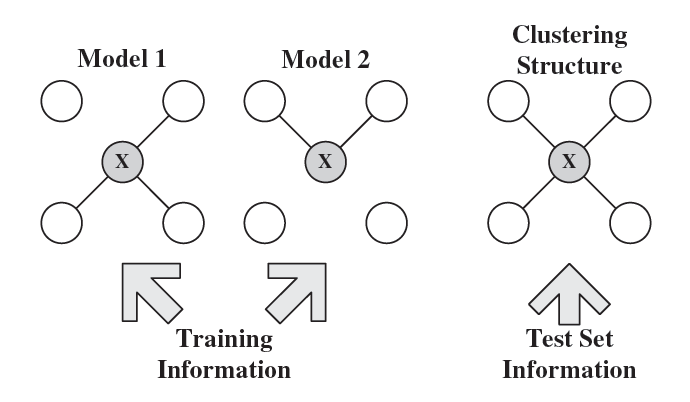
\includegraphics[width=0.75\textwidth]{similarity-approx.png}
      \caption{Example Similarity Graph Construction}
      \label{graph-construction-fig}
    \end{figure}

    Figure \ref{graph-construction-fig} depicts an example of three such graphs, where $w_{M_1,x} \propto \frac34$, and $w_{M_2,x} \propto \frac12$ since models 1 and 2 have 3 of 4 and 2 of 4 neighbors in common with $x$ on the test set respectively. With this, we can effectively weight our models to maximize their utility on a per-example basis, providing insight into the power of this framework.

    It is crucial to note that this estimation is based upon a clustering assumption \autocite{gao_fan_jiang_han_2008}, asserting that an average clustered train set must be mostly representative of the actual distribution of class labels for examples in the set. If this assumption is not fulfilled, then we simply take an evenly weighted average of the model predictions for all $x \in T$ such that
    \begin{equation} \label{weighted-model-output}
      P(y|x) = \sum_{i=1}^{k}w_{M_i, x}P(y|x, M_i)
    \end{equation}
    where $P(y|x, M_i)$ denotes the output prediction of $M_i$ for example $x$, and use $w_{M_i, x} = 1/k$ for all models.

    \begin{figure}[h]
      \centering
      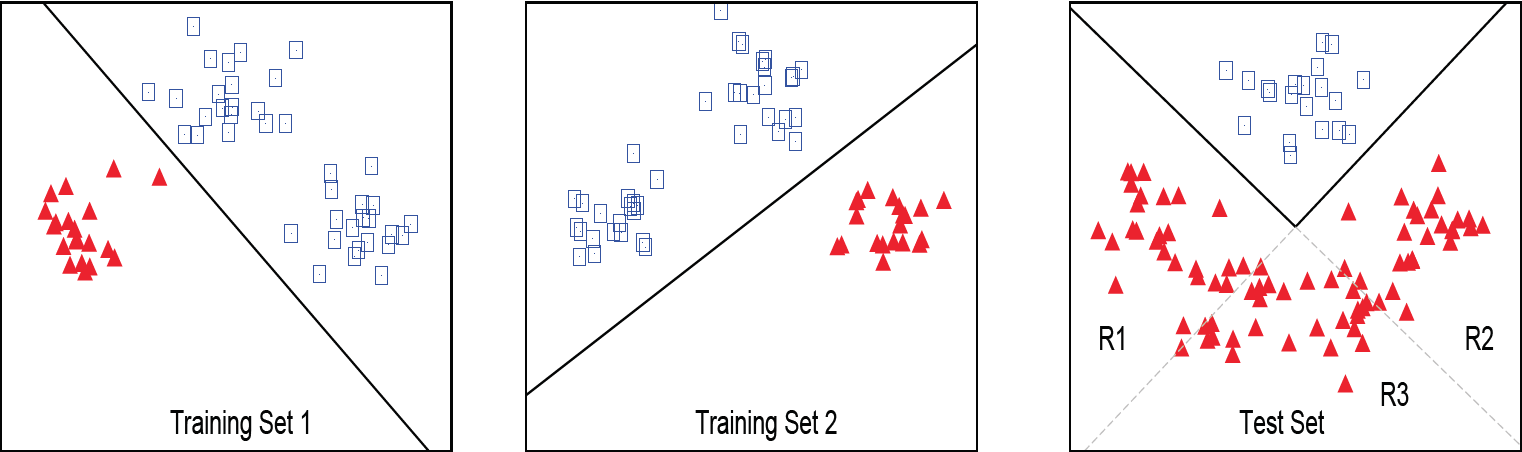
\includegraphics[width=0.75\textwidth]{toy-example.png}
      \caption{Toy Problem}
      \label{toy-data-fig}
    \end{figure}

    \section{Algorithm Implementation} \label{algorithm}
    Figure \ref{lwe-algorithm-fig} outlines the general structure which was followed for the algorithm implementation.
    \begin{figure}[h]
      \centering
      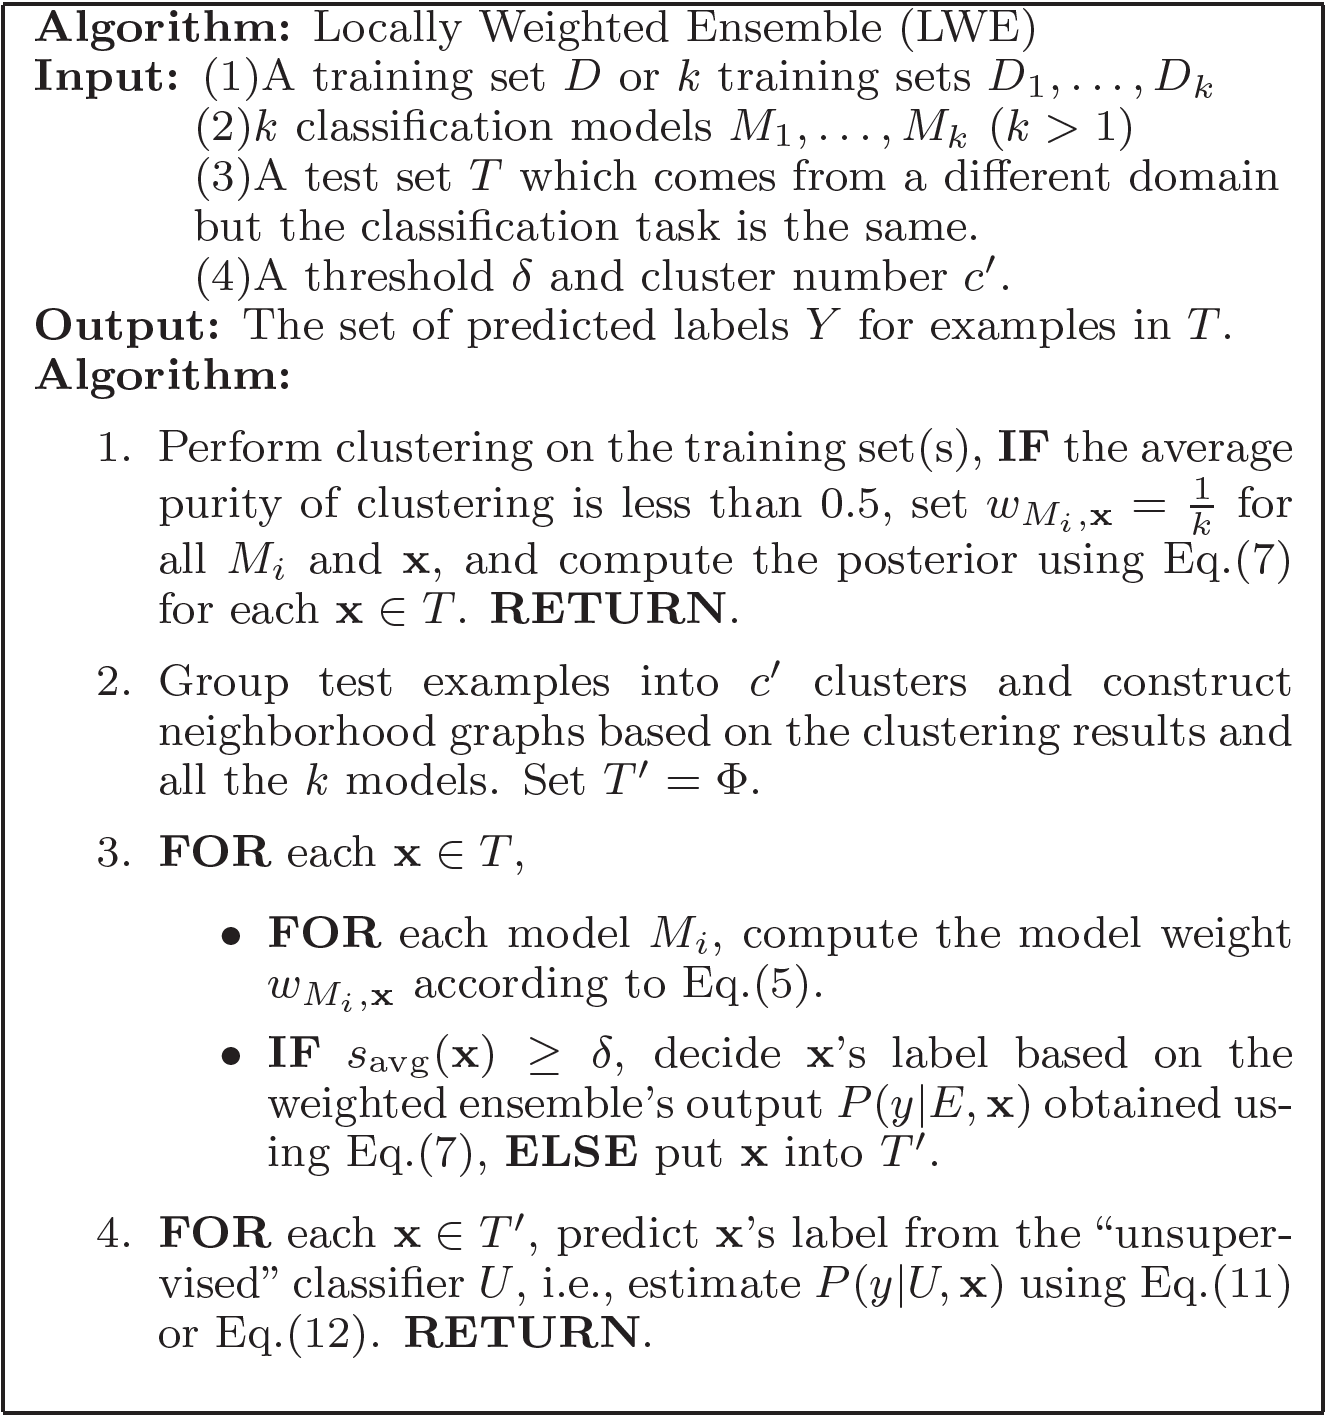
\includegraphics[width=0.5\textwidth]{lwe-algorithm.png}
      \caption{Locally Weighted Ensembling Framework}
      \label{lwe-algorithm-fig}
    \end{figure}

    We begin by training models $M_i$ corresponding to each training set $D_i$ with Logistic Regression, and pass each trained model to the function. We perform clustering on the each training set $D_i$ using \texttt{AgglomerativeClustering} from scikit-learn, and compute the confusion matrix according to the class labels for each $x \in D_i$. If the clustering assumption fails, then we cannot estimate the structure of the test domain using the structure of the training domains, so we return the average model output as demonstrated in Equation \eqref{weighted-model-output}. Otherwise, we proceed with the LWE algorithm. We cluster the testing domain and then construct neighborhood graphs as proposed in Section \ref{estimating-test-domain}.

    Using these neighborhoods, we iterate over the examples in the test domain and compute a normalized model weight \autocite{gao_fan_jiang_han_2008},
    \begin{equation}
      w_{M_i,x} = \frac{s(G_{M_i}, G_T;x)}{\sum_{i=1}^{k}s(G_{M_i}, G_T;x)}
    \end{equation}
    and if the the average $s_{avg}(x) = \frac{1}{k} \sum_{i=1}^{k}s(G_{M_i,G_T;x})$ satisfies a threshold value $\delta$, compute the output for $x$ using Equation \eqref{weighted-model-output}. Otherwise, estimate the output of $x$ by taking the average output of neighbors of $x$ which are members of the same cluster, and also have an average structural similarity $s_{avg}(x) \geq \delta$.

    This step allows us to approximate any example with reasonable accuracy regardless of a lack of confident model output, and is a significant portion of the manner in which the framework distinguishes itself from other ensembling methods, allowing us to leverage both structural similarity and model confidence for local regions of the test space.

    We have additionally implemented a baseline classifier (SGA) \autocite{gao_fan_jiang_han_2008} for comparison which simply uses the weighted output from Equation \eqref{weighted-model-output} with $w_{M_i} = 1/k$ without the clustering assumption, and a variant pLWE, which uses Equation \eqref{weighted-model-output} with the local model weight, regardless of structural similarity at $x$. We compare these approaches in Section \ref{analysis}.

    \section{Results and Analysis} \label{analysis}

    We first run the algorithm on the Multi-Domain Sentiment Dataset, consisting of Amazon Reviews. We apply training on DVD reviews to produce sentiment classification for reviews of Kitchen products, training on 1000 reviews from a single dataset and test on a set of 300 reviews, allowing for a 5000 dimensional feature space.

    \begin{figure}[h]
      \centering
      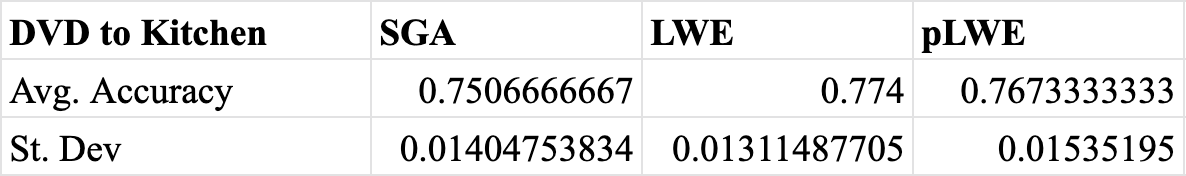
\includegraphics[width=.75\textwidth]{amazon-reviews.png}
      \caption{Amazon Review Sentiment Classification}
      \label{amazon-review-fig}
    \end{figure}

    While the classifier's accuracy is not particularly stellar, LWE manages to significantly outperform the baseline classifier, SGA, with the true mean of the difference between LWE and SGA's accuracy $\mu \in [0.0033, 0.0427]$ with 95\% confidence. However, pLWE fails to be statistically significant, with $\mu \in [-0.00447, 0.03647]$ with 95\% confidence, despite overall poor clustering quality on both the training and testing domains.


    \begin{figure}[h]
      \centering
      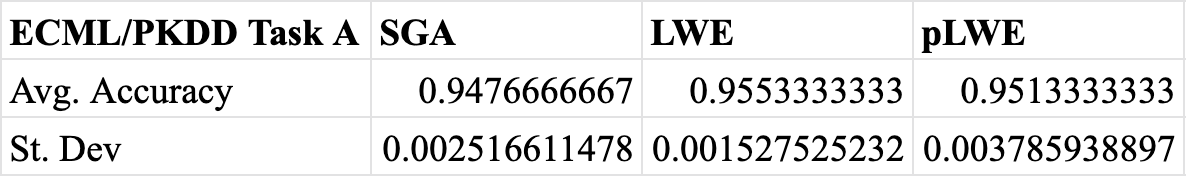
\includegraphics[width=.75\textwidth]{spam-task-a.png}
      \caption{Spam: ECMLL/PKDD Task A Results}
      \label{task-a-fig}
    \end{figure}

    Next, we run the algorithm on ECMLL/PKDD Task A and Task B, spam datasets, as described in the group paper, with results shown in Figure \ref{task-a-fig}.

    Task A has 4000 source domain examples, resulting in a high initial baseline, which is only slightly improved upon by LWE and pLWE, although the differences are weakly statistically significant.

    \begin{figure}[h]
      \centering
      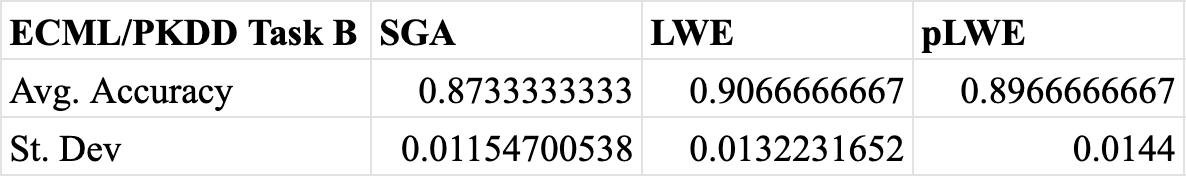
\includegraphics[width=.75\textwidth]{spam-task-b.png}
      \caption{Spam: ECMLL/PKDD Task B Results}
      \label{task-b-fig}
    \end{figure}

    Task B has 15 sets containing 100 examples each, yielding a lower base accuracy, since not all models are equally effective when training across multiple domains, yielding an inferior approach when predicting with the averaged output in Equation \eqref{weighted-model-output}. The results of LWE and pLWE are both statistically significant when compared against the base classifier as demonstrated in the group writeup.

    Finally, we run on the 20 Newsgroups dataset \autocite{gao_fan_jiang_han_2008}, yielding the best overall performance of this algorithm as demonstrated by results in Figure \ref{newsgroups-fig}.

    \begin{figure}[h]
      \centering
      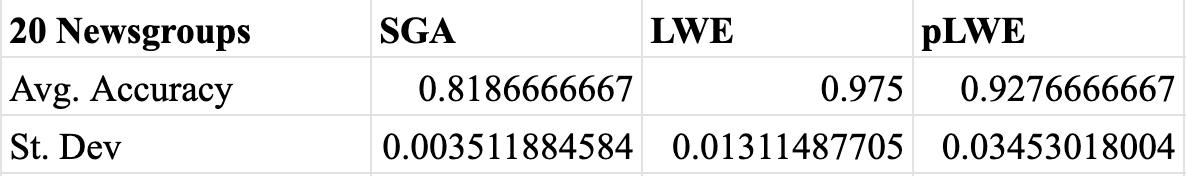
\includegraphics[width=.75\textwidth]{20-newsgroups.png}
      \caption{20 Newsgroups Results}
      \label{newsgroups-fig}
    \end{figure}

    We find this dataset to be optimal for this approach since it is extremely purely clustered, but also has substantial depth to produce highly confident classifiers for nearly any local $x \in T$, although weaker points still exist near decision boundaries, as indicated by differing accuracy between results on LWE and pLWE. The accuracy of LWE outpaces the baseline by nearly 16\%, and demonstrates one of the most effective applications of this framework in this problem space.

    \section{Comparison to Other Relevant Literature} \label{literature}

    We have explored related work detailing with an alternative approach to transform the model of training examples to produce a Bayesian prior which can be applied to the test domain \autocite{bayesian-prior}. Other approaches alternatively attempt to reduce covariate shift by reweighting training examples according to their ratio of test frequency to train frequency to minimize the reweighted probability \autocite{shimodaira_2000}. In each case, the methods fail to consider multiple source domains, and lose out on the benefit of model localization on a test domain.
    \section{Conclusions}

    We have implemented the Locally Weighted Ensembling framework, in addition to a Partially Locally Weighted variant, and a baseline classifier on which to compare performance across three datasets. In each case, the LWE framework proved to provide statistically significant performance gains, approaching 16\% accuracy improvement on some datasets.

    With this framework, we effectively outperform a standard classifier in cases where source and target domains differ, or match in cases where we deal with a standard machine learining problem. Finally, we have demonstrated the effectiveness of this approach to problems where target domain data is limited, but plentiful in other related areas, and demonstrated its utility for future use.

    \newpage
    \printbibliography
\end{document}